\documentclass[xcolor=dvipsnames,aspectratio=169,t]{beamer}
  % t means frames are vertically centered to the top
\usepackage{slides-header}
\title{Reduced Row Echelon Form}

\begin{document}
\maketitle

\begin{frame}{Solving a Linear System Using Matrices}

  {\small  Solve the following system.}
  
  {\small
   \[
   \begin{array}{l}
     x_1 +x_2 +x_3=7 \\
     x_1 -x_2 +2x_3= 7\\
     5x_1+x_2+x_3=11
  \end{array}  \sim
      \begin{bmatrix}
        1 & 1 & 1 & 7\\
        1 & -1 & 2 & 7\\
        5 & 1 & 1 & 11
      \end{bmatrix}
      \rightarrow
       \begin{bmatrix}
        1 & 1 & 1 & 7\\
        0 & -2 & 1 & 0\\
        5 & 1 & 1 & 11
      \end{bmatrix}
    \rightarrow      \]
   }

  {\small
  \[    \rightarrow 
  \begin{bmatrix}
        1 & 1 & 1 & 7\\
        0 & -2 & 1 & 0\\
        0 & -4 & -4 & -24
      \end{bmatrix}
  \rightarrow
  \begin{bmatrix}
        1 & 1 & 1 & 7\\
        0 & -2 & 1 & 0\\
        0 & 0 & -6 & -24
  \end{bmatrix}
  \rightarrow
  \begin{bmatrix}
        1 & 1 & 1 & 7\\
        0 & -2 & 1 & 0\\
        0 & 0 & 1 & 4
      \end{bmatrix}  
  \rightarrow
  \begin{bmatrix}
        1 & 1 & 1 & 7\\
        0 & -2 & 0 & -4\\
        0 & 0 & 1 & 4
      \end{bmatrix}  
  \rightarrow
  \]}

  {\small
    \[ \rightarrow
  \begin{bmatrix}
        1 & 1 & 1 & 7\\
        0 & 1 & 0 & 2\\
        0 & 0 & 1 & 4
      \end{bmatrix}  
  \rightarrow
  \begin{bmatrix}
        1 & 0 & 1 & 5\\
        0 & 1 & 0 & 2\\
        0 & 0 & 1 & 4
      \end{bmatrix}  
  \rightarrow
  \alert{\begin{bmatrix}
        1 & 0 & 0 & 1\\
        0 & 1 & 0 & 2\\
        0 & 0 & 1 & 4
      \end{bmatrix}  }
  \]}
    
\colorb{Thus $(x_1,x_2,x_3) = (1,2,4)$ is a solution of the linear system.}
  
\end{frame}


\begin{frame}{Finding a General Algorithm}
  \begin{itemize}
    \item We will build an algorithm that we can apply to the augmented matrix of any general system of linear equations, no matter how many  variables and equations the system has.
    \item The goal is to transform the augmented matrix to a special yet \alert{equivalent} form from which we can easily see the solution.
    \item We will apply \alert{elementary row operations} to transform the augmented matrix.
  \end{itemize}

  \[ 
  \begin{bmatrix}
    1 & 0 & 0 & 1\\
    0 & 1 & 0 & 2\\
    0 & 0 & 1 & 4
  \end{bmatrix}       \qquad  
  \begin{bmatrix}
    1 & 0 & -3 \\
    0 & 1 & -2
  \end{bmatrix}
  \]
  \medskip

  \bbox
    What properties do the two matrices above have in common?
  \ebox
\end{frame}

\begin{frame}{Row Echelon Form}

  \bbox
  A matrix is in \colorb{row echelon form} if it has the following properties:
  \bb
  \ii All nonzero rows are above any rows of all zeros.
  \ii Each \colorb{leading entry} (ie, the leftmost nonzero entry) is in a column to the right of the leading entry of the row above it.
  \ii All entries in a column below a leading entry are zeros.
  \ee
  \ebox

  \renewcommand{\p}{\colorr{\blacksquare}}  % pivot
  \newcommand{\n}{\colorb{*}}  % possibly nonzero
  \[
    \begin{bmatrix}
      \p & \n & \n & \n \\
       0 & \p & \n & \n \\
       0 &  0 &  0 &  0 \\
       0 &  0 &  0 &  0
    \end{bmatrix}
    \qquad
    \begin{bmatrix}
      0 & \p & \n & \n & \n & \n & \n & \n & \n & \n \\
      0 &  0 &  0 & \p & \n & \n & \n & \n & \n & \n \\
      0 &  0 &  0 &  0 & \p & \n & \n & \n & \n & \n \\
      0 &  0 &  0 &  0 &  0 & \p & \n & \n & \n & \n \\
      0 &  0 &  0 &  0 &  0 &  0 &  0 &  0 & \p & \n
    \end{bmatrix}
  \]
  
\end{frame}
  
\begin{frame}{Reduced Row Echelon Form}

  \bbox
  If a matrix is in row echelon form satisfies the following two additional conditions, then it is in \colorb{reduced row echelon form (RREF)}.
  \bb
  \addtocounter{enumi}{3}
  \ii The leading entry in each nonzero row is $1$.
  \ii Each leading $1$ is the only entry in its column.
  \ee
  \ebox

  \medskip
  
  {\small
  \[
    \renewcommand{\p}{\colorr{\blacksquare}}  % pivot
    \newcommand{\n}{\colorb{*}}  % possibly nonzero
    \begin{bmatrix}
      0 & \p & \n & \n & \n & \n & \n & \n & \n & \n \\
      0 &  0 &  0 & \p & \n & \n & \n & \n & \n & \n \\
      0 &  0 &  0 &  0 & \p & \n & \n & \n & \n & \n \\
      0 &  0 &  0 &  0 &  0 & \p & \n & \n & \n & \n \\
      0 &  0 &  0 &  0 &  0 &  0 &  0 &  0 & \p & \n
    \end{bmatrix}
    \qquad
    \renewcommand{\p}{\colorr{\mathbf{1}}}  % pivot
    \begin{bmatrix}
      0 & \p & \n &  0 &  0 &  0 & \n & \n &  0 & \n \\
      0 &  0 &  0 & \p &  0 &  0 & \n & \n &  0 & \n \\
      0 &  0 &  0 &  0 & \p &  0 & \n & \n &  0 & \n \\
      0 &  0 &  0 &  0 &  0 & \p & \n & \n &  0 & \n \\
      0 &  0 &  0 &  0 &  0 &  0 &  0 &  0 & \p & \n
    \end{bmatrix}
  \]
  }
  \medskip

  Which \alert{elementary row operations} can be applied to the matrix on the left to express it in reduced row echelon form?
\end{frame}

\begin{frame}{Echelon Formation}

  \begin{columns}[T]
    \column{0.4\tw}
    
  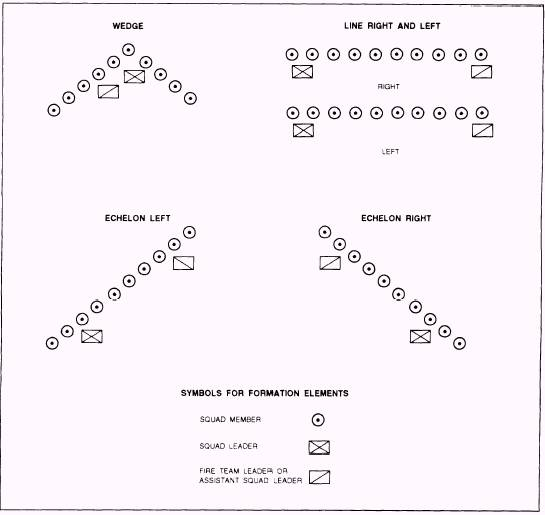
\includegraphics[width=0.95\tw]{images/fig-echelon-troops.jpg}

  \column{0.6\tw}
  
\begin{quote}
  An \colorb{echelon formation} is a (usually military) formation in which its units are arranged diagonally. Each unit is stationed behind and to the right (a ``right echelon''), or behind and to the left (``left echelon''), of the unit ahead. The name of the formation comes from the French word echelon, meaning a rung of a ladder, which describes the shape that this formation has when viewed from above or below.
\end{quote}
\hspace*{7em} -- Source: Wikipedia

\end{columns}

\vfill


{\footnotesize Image Credit:  \colorb{\href{https://thefreelancehistorywriter.com/2012/10/27/the-battle-of-flodden/}{https://thefreelancehistorywriter.com/2012/10/27/the-battle-of-flodden/}}}
  
  \end{frame}

\begin{frame}{Constructing an Algorithm}

  \begin{columns}[T]
    
    \column{0.65\tw}
 We now construct an algorithm using \alert{elementary row operations} to express any nonzero matrix into an equivalent reduced row echelon.

\column{0.35\tw}
 
\[ \begin{bmatrix} 0 & -3 & -6 & 4 & 9\\
  -1 & -2 & -1 & 3 & 1 \\
  -2 & -3 & 0 & 3 & -1\\
1 & 4 & 5 & -9 & -7 \end{bmatrix} \]

  \end{columns}

\begin{columns}[c]
    
    \column{0.65\tw}
  
 \bb
 \ii Begin with the leftmost nonzero column (called the \alert{pivot column}).

 \ii Select a nonzero entry in the pivot column as a \alert{pivot}. 
  If necessary, swap rows so this entry is in the top row.

 

 \ee

\column{0.35\tw}

\[ \begin{bmatrix}   \colorb{1} & 4 & 5 & -9 & -7\\
  -1 & -2 & -1 & 3 & 1 \\
  -2 & -3 & 0 & 3 & -1\\
0 & -3 & -6 & 4 & 9  \end{bmatrix} \]

%%\ii   $\dsty \begin{bmatrix}   1 & 4 & 5 & -9 & -7\\
%   0 & 2 & 4 & -6 & -6\\
 %  0 & 5 & 10 & -15 & -15\\
%0 & -3 & -6 & 4 & 9  \end{bmatrix} $

\end{columns}

\end{frame}

\begin{frame}{Constructing an Algorithm}

  \[ \begin{bmatrix}   \colorb{1} & 4 & 5 & -9 & -7\\
  -1 & -2 & -1 & 3 & 1 \\
  -2 & -3 & 0 & 3 & -1\\
0 & -3 & -6 & 4 & 9  \end{bmatrix} \]

  
  \bb
  \setcounter{enumi}{2}
 \ii Add multiples of the row with the pivot to create zeros in all positions below the pivot.

 \[ \begin{bmatrix}   1 & 4 & 5 & -9 & -7\\
  0 & 2 & 4 & -6 & -6 \\
  0 & 5 & 10 & -15 & -15\\
0 & -3 & -6 & 4 & 9  \end{bmatrix} \]

 \ee

 \end{frame}

\begin{frame}{Constructing an Algorithm}

  {\small
 \[ \begin{bmatrix}   1 & 4 & 5 & -9 & -7\\
  0 & \colorb{2} & \alert{4} & \alert{-6} & \alert{-6} \\
  0 & \alert{5} & \alert{10} & \alert{-15} & \alert{-15}\\
0 & \alert{-3} & \alert{-6} & \alert{4} & \alert{9}  \end{bmatrix} \] }

 \bb
 \setcounter{enumi}{3}

\ii Ignore the row containing the pivot position and consider the remaining submatrix.
  Repeat steps 1-3 above to the remaining submatrix.
  Repeat this process on each successive submatrix until there are no more nonzero rows to modify.

{\small 
\[ \begin{bmatrix}   \colorb{1} & 4 & 5 & -9 & -7\\
  0 & \colorb{2} & 4 & -6 & -6 \\
  0 & 0 & 0 & 0 & 0\\
  0 & 0 & 0 & \alert{-5} & 0  \end{bmatrix}
\rightarrow
\begin{bmatrix}   \colorb{1} & 4 & 5 & -9 & -7\\
  0 & \colorb{2} & 4 & -6 & -6 \\
  0 & 0 & 0 & \colorb{-5} & 0 \\
  0 & 0 & 0 & 0 & 0 \end{bmatrix}
\] }

\ee

The matrix is in row echelon form, but we want to continue to express the matrix in reduced row echelon form.
\end{frame}

\begin{frame}{Constructing an Algorithm}

 \[ \begin{bmatrix}   \colorb{1} & 4 & 5 & -9 & -7\\
  0 & \alert{2} & 4 & -6 & -6 \\
  0 & 0 & 0 & \colorg{-5} & 0 \\
  0 & 0 & 0 & 0 & 0 \end{bmatrix}
 \rightarrow
  \begin{bmatrix}   \colorb{1} & 4 & 5 & -9 & -7\\
  0 & \alert{1} & 2 & -3 & -3 \\
  0 & 0 & 0 & \colorg{1} & 0 \\
  0 & 0 & 0 & 0 & 0 \end{bmatrix}
 \]

\bb
\setcounter{enumi}{4}
\ii Scale each row so the pivot in the row is $1$.
\ii Beginning with the rightmost pivot, add multiples of that row to create zeros in all positions above it. Then move to the next pivot to the left and repeat until the matrix is in reduced row echelon form.

 \[ \begin{bmatrix}   
  \colorb{1} & \alert{4} & 5 & \colorg{0} & -7\\
  0 & \alert{1} & 2 & \colorg{0} & -3 \\
  0 & 0 & 0 & \colorg{1} & 0 \\
  0 & 0 & 0 & 0 & 0 \end{bmatrix}
 \rightarrow
 \begin{bmatrix}   
  \colorb{1} & \alert{0} & -3 & \colorg{0} & 5\\
  0 & \alert{1} & 2 & \colorg{0} & -3 \\
  0 & 0 & 0 & \colorg{1} & 0 \\
  0 & 0 & 0 & 0 & 0 \end{bmatrix}
  \]
 \ee

\end{frame}

\begin{frame}{Gaussian Elimination}

  {\small
  The series of elementary row operations outlined in the previous slides is a algorithm that when applied to any nonzero matrix (no matter how big) will result in a reduced row echelon matrix that is row equivalent to the original matrix.
  
  \begin{enumerate}
    \item Begin with the leftmost nonzero column (called the \alert{pivot column}).
    \item Select a nonzero entry in the pivot column as a \alert{pivot}. If necessary, swap rows so this entry is on the top row.
    \item Add multiples of the row with the pivot to create zeros in all positions below the pivot.  
    \item Ignore the row containing the pivot position and consider the remaining submatrix. Repeat steps 1-3 above to the remaining submatrix. Repeat this process on each successive submatrix until there are no more nonzero rows to modify.
    \item Scale each row so the pivot in the row is $1$.
    \item Beginning with the rightmost pivot, add multiples of that row to create zeros in all positions above it. Then move to the next pivot to the left and repeat until the matrix is in reduced row echelon form.
  \end{enumerate}

This process is called \alert{Gaussian Elimination}. }

\end{frame}

\begin{frame}{Existence and Uniqueness of RREF}

  {\small
  \bi
  \ii \alert{Existence:} Given any matrix, we can apply a series of elementary row operations to find an equivalent matrix in reduced row echelon form.
  \ii The series of elementary row operations that we apply is not unique, but the end result is \alert{unique}.
  \ei }
  
  {\small
  \[ \begin{bmatrix}
    0 & 1 & -2\\
    -2& -2& -4 \\
    1 & 1 & 2 
  \end{bmatrix}
  \rightarrow
  \colorb{
 \begin{bmatrix}
    -2& -2& -4 \\
  0 & 1 & -2\\
    1 & 1 & 2 
  \end{bmatrix}
  \rightarrow
 \begin{bmatrix}
    1& 1& 2 \\
    0 & 1 & -2\\
    1 & 1 & 2 
  \end{bmatrix}
  \rightarrow
 \begin{bmatrix}
    1& 1& 2 \\
    0 & 1 & -2\\
    0 & 0 & 0 
  \end{bmatrix} }
 \rightarrow
 \begin{bmatrix}
    1& 0& 4 \\
    0 & 1 & -2\\
    0 & 0 & 0 
  \end{bmatrix} 
 \] }


{\small  
  \[ \begin{bmatrix}
    0 & 1 & -2\\
    -2& -2& -4 \\
    1 & 1 & 2 
  \end{bmatrix}
  \rightarrow
\alert{ 
  \begin{bmatrix}
    1 & 1 & 2 \\
   -2 & -2 & -4 \\
    0 & 1 & -2
    \end{bmatrix}
 \rightarrow
  \begin{bmatrix}
    1 & 1 & 2 \\
    0 & 0 & 0 \\
    0 & 1 & -2
    \end{bmatrix}
\rightarrow
 \begin{bmatrix}
  1 & 1 & 2 \\
  0 & 1 & -2 \\
  0& 0& 0
  \end{bmatrix}
  }
  \rightarrow
 \begin{bmatrix}
    1 & 0 & 4 \\
    0 & 1 & -2 \\
    0& 0& 0
 \end{bmatrix} \] }

  \begin{theorem}[Uniqueness of Reduced Row Echelon Form]
    Every matrix is equivalent to one and only one matrix in reduced row echelon form.
  \end{theorem}

\end{frame}

\begin{frame}{Example 1}

  \begin{columns}[T]

    \column{0.4\tw}
    
  Find a solution to the system
  
  \[
  \begin{array}{ccccccc}
    2x_1 & + & x_2 & + & x_3&=&5\\
    4x_1 & - & 6x_2 & & &=&-2\\
    -2x_1 & + & 7x_2 & + & 2x_3 &=& 9
  \end{array}
  \]

\bb
\ii Set up the augmented matrix:
\ee

\[ \begin{bmatrix}
  2 & 1 & 1 & 5\\
  4 & -6 & 0 & -2\\
  -2 & 7 & 2 & 9
\end{bmatrix} \]

\column{0.6\tw}

\bb
\setcounter{enumi}{1}

\ii Apply the row reduction algorithm and express the matrix in reduced row echelon form (RREF).
\ee

\[ \begin{bmatrix}
  2 & 1 & 1 & 5\\
  4 & -6 & 0 & -2\\
  -2 & 7 & 2 & 9
\end{bmatrix}
\rightarrow
 \begin{bmatrix}
 \alert{1} & 0.5 & 0.5 & 2.5\\
  4 & -6 & 0 & -2\\
  -2 & 7 & 2 & 9
 \end{bmatrix}
 \rightarrow \ldots \]


\end{columns}

\end{frame}

\begin{frame}{Solution}

  {\small 
\[ \begin{bmatrix}
  2 & 1 & 1 & 5\\
  4 & -6 & 0 & -2\\
  -2 & 7 & 2 & 9
\end{bmatrix}
\rightarrow
 \begin{bmatrix}
  \alert{1} & 0.5 & 0.5 & 2.5\\
  4 & -6 & 0 & -2\\
  -2 & 7 & 2 & 9
 \end{bmatrix}
 \rightarrow 
 \begin{bmatrix}
  \alert{1} & 0.5 & 0.5 & 2.5\\
  0 & -8 & -2 & -12\\
  -2 & 7 & 2 & 9
 \end{bmatrix}
 \rightarrow 
 \begin{bmatrix}
  \alert{1} & 0.5 & 0.5 & 2.5\\
  0 & \colorb{-8} & -2 & -12\\
  0 & 8 & 3 & 14
 \end{bmatrix}
 \rightarrow 
 \] }

{\small
  \[ \rightarrow
 \begin{bmatrix}
  \alert{1} & 0.5 & 0.5 & 2.5\\
  0 & \colorb{-8} & -2 & -12\\
  0 & 0 & \colorg{1} & 2
 \end{bmatrix}
\rightarrow
\begin{bmatrix}
  \alert{1} & 0.5 & 0.5 & 2.5\\
  0 & \colorb{1} & 0.25 & 1.5\\
  0 & 0 & \colorg{1} & 2
\end{bmatrix}
\rightarrow
\begin{bmatrix}
  \alert{1} & 0.5 & 0.5 & 2.5\\
  0 & \colorb{1} & 0 & 1\\
  0 & 0 & \colorg{1} & 2
\end{bmatrix}
\rightarrow
\]
}

{\small
  \[ \rightarrow
  \begin{bmatrix}
  \alert{1} & 0.5 & 0 & 1.5\\
  0 & \colorb{1} & 0 & 1\\
  0 & 0 & \colorg{1} & 2
\end{bmatrix}
\rightarrow
\begin{bmatrix}
  \alert{1} & 0 & 0 & \alert{1}\\
  0 & \colorb{1} & 0 & \colorb{1}\\
  0 & 0 & \colorg{1} & \colorg{2}
\end{bmatrix}
\mbox{ which gives }
\left\{ \begin{array}{l}
  \alert{x_1 = 1}\\
  \colorb{x_2 = 1} \\ 
  \colorg{x_3 = 2} \end{array} \right. \]
}

\end{frame}

\begin{frame}{Checking Your Solution}

  \begin{columns}[T]

    \column{0.4\tw}
    
  Find a solution to the system
  
\[   \begin{array}{ccccccc}
    2\alert{x_1} & + & \colorb{x_2} & + & \colorg{x_3}&=&5\\
    4\alert{x_1} & - & 6\colorb{x_2} & & &=&-2\\
    -2\alert{x_1} & + & 7\colorb{x_2} & + & 2\colorg{x_3} &=& 9
  \end{array}  \]

\bb
\ii Set up the augmented matrix:
\ee

\[ \begin{bmatrix}
  2 & 1 & 1 & 5\\
  4 & -6 & 0 & -2\\
  -2 & 7 & 2 & 9
\end{bmatrix} \]

\column{0.6\tw}

\bb
\setcounter{enumi}{1}

\ii Apply the row reduction algorithm and express the matrix in reduced row echelon form (RREF).

\[ \begin{bmatrix}
  2 & 1 & 1 & 5\\
  4 & -6 & 0 & -2\\
  -2 & 7 & 2 & 9
\end{bmatrix}
\sim \begin{bmatrix}
  \alert{1} & 0 & 0 & \alert{1}\\
  0 & \colorb{1} & 0 & \colorb{1}\\
  0 & 0 & \colorg{1} & \colorg{2}
\end{bmatrix}
\mbox{ or }
\left\{ \begin{array}{l}
  \alert{x_1 = 1}\\
  \colorb{x_2 = 1} \\ 
  \colorg{x_3 = 2} \end{array} \right. \]

\ii Verify your solution!

\[   \begin{array}{ccccccc}
    2\alert{(1)} & + & \colorb{1} & + & \colorg{2}&=&5\\
    4\alert{(1)} & - & 6\colorb{(1)} & & &=&-2\\
    -2\alert{(1)} & + & 7\colorb{(1)} & + & 2\colorg{(2)} &=& 9
  \end{array}  \]

\ee

\end{columns}

\end{frame}

\begin{frame}{Example 2}

  Find a solution to the system
  
\[   \begin{array}{ccccccc}
    x_1 & + & 2x_2 & + & x_3&=&-2\\
    x_1 & + & 3x_2 & - & 2x_3 &=& 1
\end{array}  % \qquad
%\begin{bmatrix}
%  1 & 2 & 1 & -2 \\
%  1 & 3 & -2 & 1
%  \end{bmatrix}
\]

\vfill

%\end{frame}

%\begin{frame}{Example 2 Solution}
We set up the augmented matrix and perform elementary row operations:
\[ \begin{bmatrix}
  \alert{1} & 2 & 1 & -2 \\
  1 & 3 & -2 & 1
  \end{bmatrix} \rightarrow
\begin{bmatrix}
  \alert{1} & 2 & 1 & -2 \\
  0 & \colorb{1} & -3 & 3
\end{bmatrix} \rightarrow
\begin{bmatrix}
  \alert{1} & 0 & 7 & -8  \\
  0 & \colorb{1} & -3 & 3
  \end{bmatrix} \]

\vfill

This gives the solution set:
\[  \begin{array}{ccccccc}
    \alert{x_1} &  & & + & 7x_3&=&-8\\
     &  & \colorb{x_2} & - & 3x_3 &=& 3
\end{array}
\mbox{ or }
\left\{ \begin{array}{l}
  \alert{x_1} = -8 - 7x_3\\
  \colorb{x_2} = 3+3x_3 \\ 
  x_3 \mbox{ is free}  \end{array} \right. \]

\end{frame}

\begin{frame}{Solutions of Linear Systems}

We have   
\[   \begin{array}{ccccccc}
    x_1 & + & 2x_2 & + & x_3&=&-2\\
    x_1 & + & 3x_2 & - & 2x_3 &=& 1
\end{array}
\mbox{ with solution }
\left\{ \begin{array}{l}
  \alert{x_1} = -8 - 7x_3\\
  \colorb{x_2} = 3+3x_3 \\ 
  x_3 \mbox{ is free}  \end{array} \right. \]

  \begin{itemize}
  \item The variables $x_1$ and $x_2$ correspond to pivot columns and are called \alert{basic variables}.
  \item The variable $x_3$ is called a \alert{free variable}.
  \item Any choice of a real number for each free variable gives a solution to the system by solving for the basic variables.\\\smallskip
  \quad For example,
    $x_3=1$ gives $\colorr{x_1}=-8-7(1)=-15$ and $\colorb{x_2}=3+3(1)=6$.\\
  \quad Thus, $(x_1,x_2,x_3)=(-15,6,1)$ is a solution to the system.
  \smallskip
  \pause
  \item If there is at least one free variable, then there are an \colorb{infinite number} of solutions.
  \end{itemize}

\end{frame}

\begin{frame}{Example 3}
  
  Find a solution to the system
\[   \begin{array}{ccccccc}
     &  & x_2 & + &2 x_3&=&0\\
    x_1 & + & 2x_2 & + & 3x_3 &=& 1\\
    x_1 & + & x_2 & + & x_3 &=& 2
\end{array}  \]

\pause

\vfill

We set up the augmented matrix and perform elementary row operations:

{\small
\[ \begin{bmatrix}
  0 & 1 & 2 & 0\\
  1 & 2 & 3 & 1\\
  1 & 1 & 1 & 2
\end{bmatrix} \rightarrow
\begin{bmatrix}
 \colorb{1} & 1 & 1 & 2 \\
  1 & 2 & 3 & 1\\
   0 & 1 & 2 & 0
 \end{bmatrix}  \rightarrow
\begin{bmatrix}
 \colorb{1} & 1 & 1 & 2 \\
  0 & \colorb{1} & 2 & -1\\
   0 & 1 & 2 & 0
 \end{bmatrix}  \rightarrow
\begin{bmatrix}
 \colorb{1} & 1 & 1 & 2 \\
  0 & \colorb{1} & 2 & -1\\
   0 & 0 & 0 & \alert{1}
\end{bmatrix} \rightarrow
\begin{bmatrix}
 \colorb{1} & 0 & -1 & 0 \\
  0 & \colorb{1} & 2 & 0\\
   0 & 0 & 0 & \alert{1}
 \end{bmatrix}  \] }

  \vfill

  This is an \alert{inconsistent} system:
  \[  \begin{array}{ccccccc}
    \colorb{x_1} &  & & - & x_3&=&0\\
    &  & \colorb{x_2} & + & 2x_3 &=& 0\\
    &  &  &  & \alert{0} &\alert{=}& \alert{1}
    \end{array}  \qquad \mbox{\alert{No Solution Exists.}}\]

\end{frame}

\begin{frame}{Summary}

  \bbox
  Given a system of linear equations:

  \bb
  \ii Write the augmented matrix of the system.
  \ii Use elementary row operations to obtain an equivalent row echelon matrix.
  \bb[(a)]
  \ii If the last (rightmost) column is a pivot column, then the system is \alert{inconsistent}. No solution exists.
  \ii If the rightmost column is not a pivot column, then the system is \colorb{consistent} and has a solution.
  \ee
  \ii Continue row reduction to obtain the reduced row echelon form (RREF).
  \ii Write the system of equations corresponding to the RREF matrix.
  \ii Rewrite each nonzero equation from the previous step so that the basic variable in the equation is expressed in terms of the free variables.
  \ee
  \ebox

  \end{frame}

\begin{frame}{Describe the Solution Set}
  If a system of linear equations has augmented matrix that is equivalent the given reduced row echelon form, give the solution set.
   
  \bb
  \ii $\dsty \begin{bmatrix}
    1 & 2 & 0 & 0 & -4 & 0 \\
    0 & 0 & 1 & 0 & 7 & 1 \\
    0 & 0 & 0 & 1 & 5 & 2 \\
    0 & 0 & 0 & 0 & 0 & 0
  \end{bmatrix}$

  \vfill
  
  \ii  $\dsty \begin{bmatrix}
    1 & 0 & -3 & -4 & 3  \\
    0 & 1 & -8 & 5 & 7  \\
    0 & 0 & 0 &  0 & 1 \\
   \end{bmatrix}$
  \ee

\end{frame}

\end{document}
